
\section{Transformer and Attention}

The Transformer is a mechanism that is based entirely on Attention. This is not the attention explored in the Sequence to Sequence model in Chapter 1. It is a model that uses no recurrent components and no convolution components. 

Recurrent components have some negative qualities. Recurrent components are hard to run with batch input data. Also they do not work with very long data strings. 

If a batch of data is to be cycled through a recurrent component, all that data has to go through the component at the first cardinal position before it is cycled through the second or third position. In the first time step everything needs to go through the first RNN module. Then the data can be moved along to the second RNN  module in the second time step.

Also because the RNN is so heavy with Neural Network components, many weights and biases, though they can remember patterns, they loose some information with every pass. This is why there is a practical limit to the length of the input sequences that the typical RNN can use. This is why the length of sentences in network models that use the RNN are limited in length.

Transformers use no RNN components. Their operations can be parallelized so that large batches of data can be processed at once during the same time step. 

Longer sequences can be considered as well, so Transformer input can contain english language sentences and even paragraphs.

\subsection*{Model Overview}
Attention mechanisms are used in a similar way in three places in the model. The first implementation of the Self Attention is discussed below.


\subsection*{Self Attention}

The Transformer has a signature self-attention mechanism. This is possibly one third of the entire Transformer mechanism. 



\begin{figure}[H]
	\begin{center}
		
	
	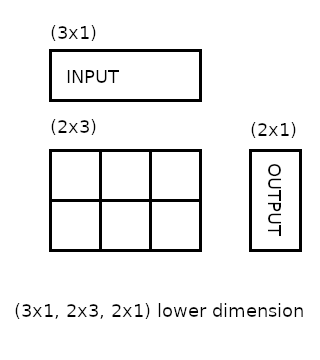
\includegraphics[scale=0.5]{diagram-mat01}
\end{center}
	\caption[Lowering Dimensionality]{Lowering Dimensionality}
	
	%\addcontentsline{lof}{section}{Loss and Accuracy}
\end{figure}

\begin{figure}[H]
	\begin{center}
		
	
	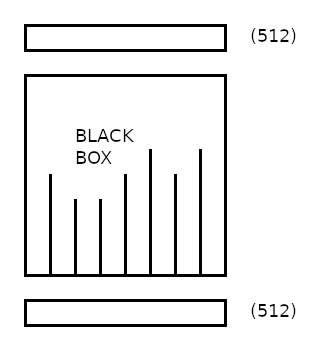
\includegraphics[scale=0.5]{diagram-mat02}
\end{center}
	\caption[Matching Input and Output]{Matching Input and Output}
	
	%\addcontentsline{lof}{section}{Loss and Accuracy}
\end{figure}

\begin{figure}[H]
	\begin{center}
		
	
	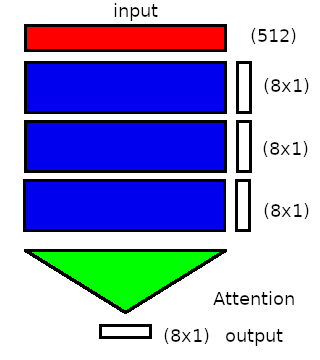
\includegraphics[scale=0.5]{diagram-mat03}
\end{center}
	\caption[Attention Output]{Attention Output}
	
	%\addcontentsline{lof}{section}{Loss and Accuracy}
\end{figure}